\documentclass{article}
\usepackage[UTF8]{ctex}
\usepackage{pythonhighlight}
\usepackage{markdown}
\usepackage{listings}
\lstset{
    basicstyle          =   \tt,          % 基本代码风格
    identifierstyle=\color{brown!80!black},
    keywordstyle        =   \color{purple}\bfseries,          % 关键字风格
    commentstyle        =   \rmfamily\itshape,  % 注释的风格,斜体
    stringstyle         =   \ttfamily,  % 字符串风格
    flexiblecolumns,                % 别问为什么,加上这个
    numbers             =   left,   % 行号的位置在左边
    showspaces          =   false,  % 是否显示空格,显示了有点乱,所以不现实了
    numberstyle         =   \zihao{-5}\ttfamily,    % 行号的样式,小五号,tt等宽字体
    showstringspaces    =   false,
    captionpos          =   t,      % 这段代码的名字所呈现的位置,t指的是top上面
    frame               =   lrtb,   % 显示边框
    backgroundcolor=\color[RGB]{245,245,244},
}


% Language setting
% Replace `english' with e.g. `spanish' to change the document language
\usepackage[english]{babel}
\usepackage{float}
% Set page size and margins
% Replace `letterpaper' with `a4paper' for UK/EU standard size
\usepackage[letterpaper,top=2cm,bottom=2cm,left=3cm,right=3cm,marginparwidth=1.75cm]{geometry}

% Useful packages
\usepackage{amsmath}
\usepackage{graphicx}
\usepackage[colorlinks=true, allcolors=blue]{hyperref}

\title{数逻实验报告Lab9}
\author{雷远航}

\begin{document}

\maketitle

\begin{abstract}
    锁存器与触发器基本原理
\end{abstract}


\section*{一:操作方法与实验步骤}

\subsection*{1. SR锁存器}
    \begin{figure}[H]
    \centering
    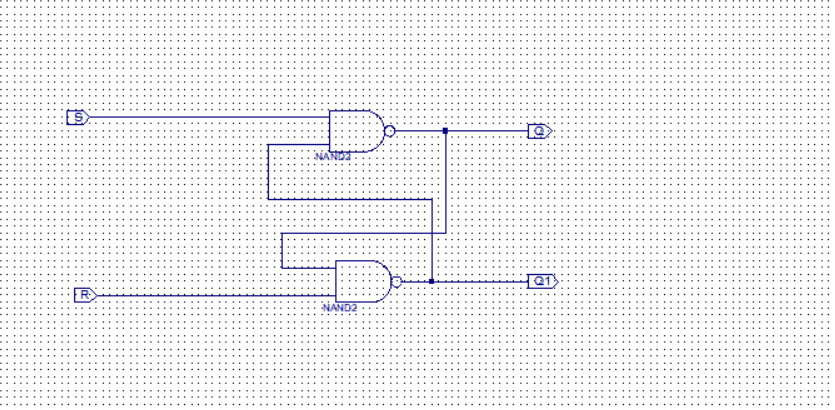
\includegraphics[width=0.9\textwidth]{lab9p/5.png}
    \caption{\label{Lab9}SR锁存器}
    \end{figure}
\subsubsection*{SR\_LATCH仿真代码initial块}
    \begin{figure}[H]
    \centering
    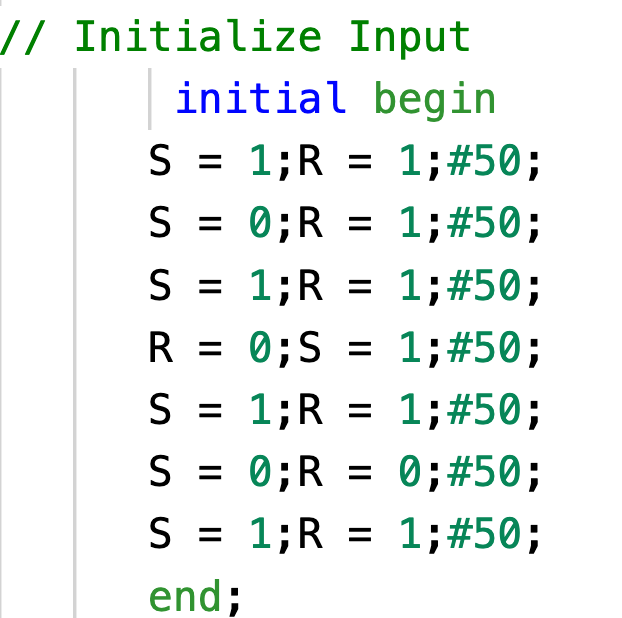
\includegraphics[width=0.4\textwidth]{lab9p/11.png}
    \caption{\label{Lab9}initial块}
    \end{figure}


\subsection*{2. 门控SR锁存器}
    \begin{figure}[H]
    \centering
    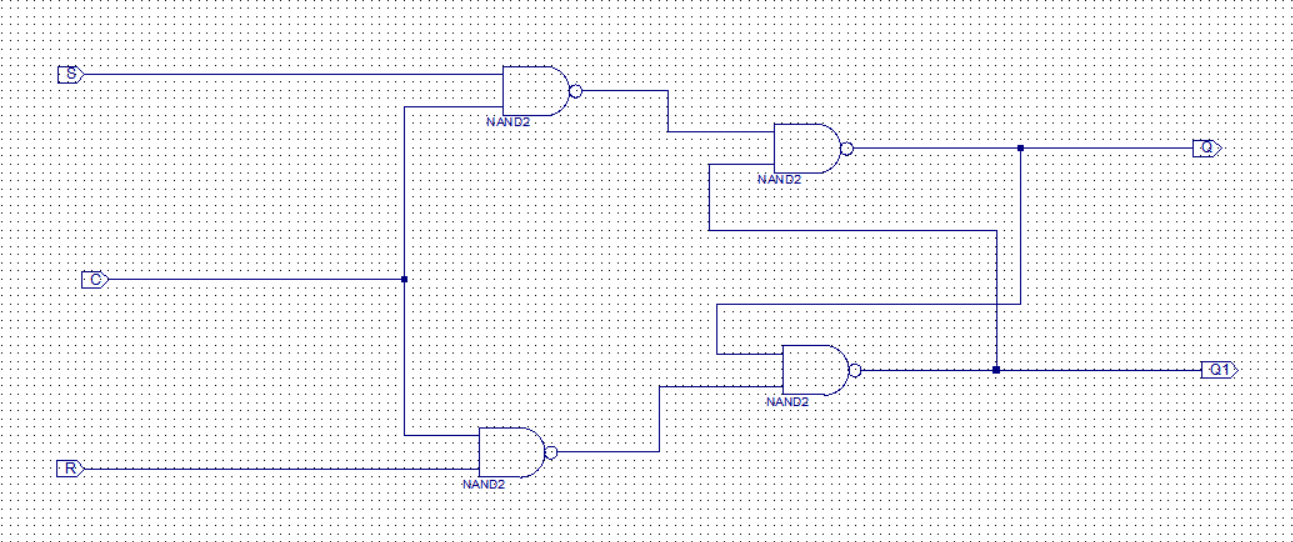
\includegraphics[width=0.9\textwidth]{lab9p/6.png}
    \caption{\label{Lab9}门控SR锁存器}
    \end{figure}

\subsubsection*{门控SR\_LATCH仿真代码initial块}
    \begin{figure}[H]
    \centering
    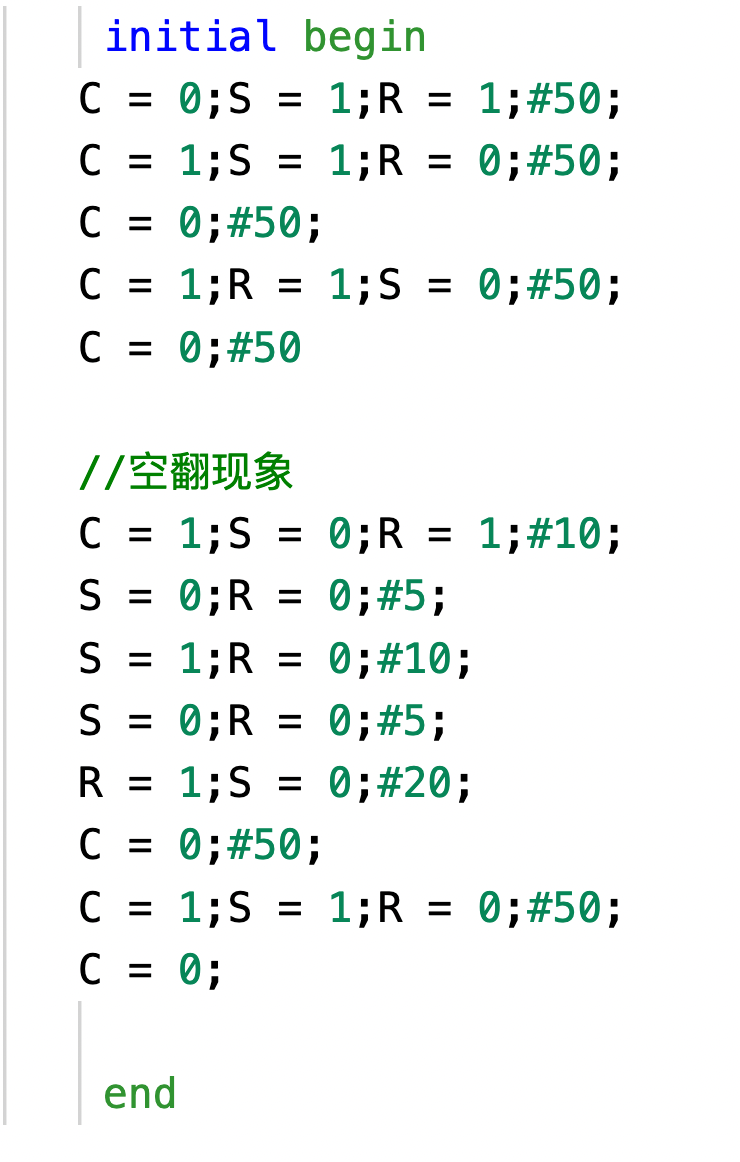
\includegraphics[width=0.4\textwidth]{lab9p/12.png}
    \caption{\label{Lab9}initial块}
    \end{figure}

\subsection*{3. D锁存器}
    \begin{figure}[H]
    \centering
    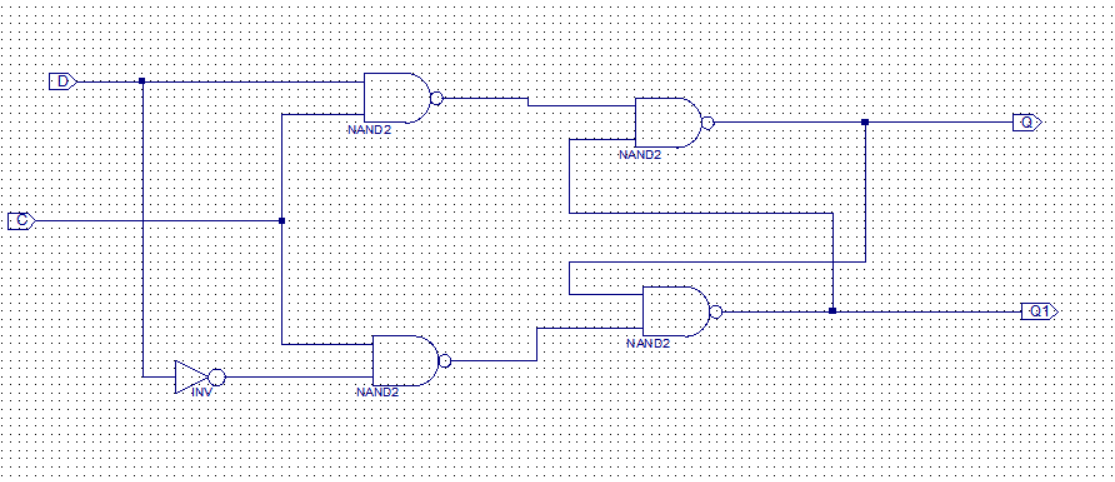
\includegraphics[width=0.9\textwidth]{lab9p/7.png}
    \caption{\label{Lab9}D锁存器}
    \end{figure}

\subsubsection*{门控D\_LATCH仿真代码initial块}
    \begin{figure}[H]
    \centering
    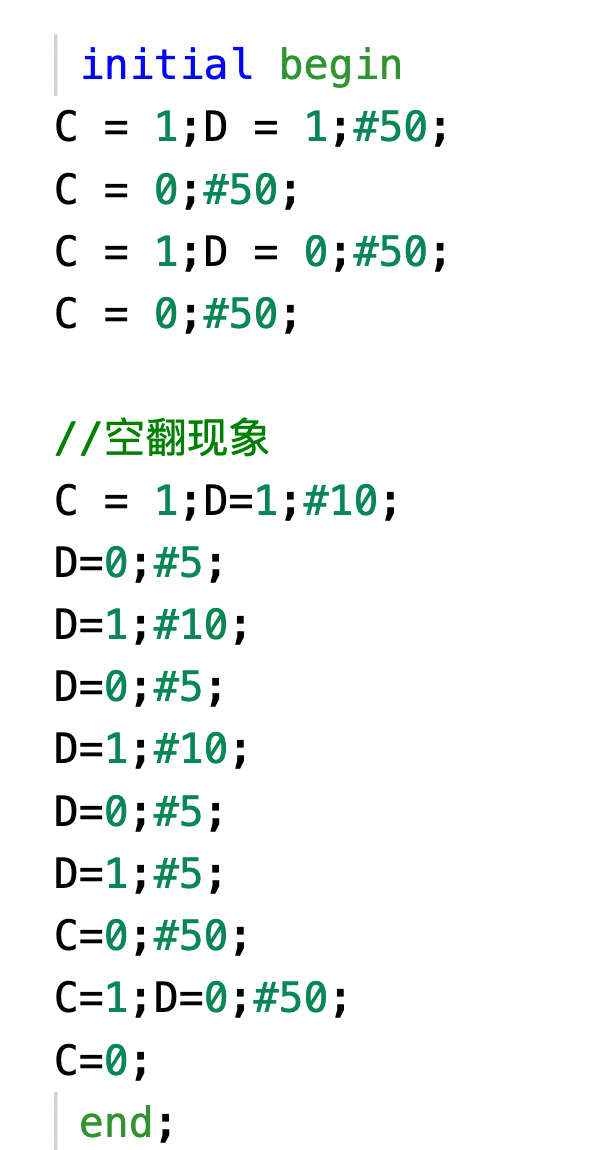
\includegraphics[width=0.3\textwidth]{lab9p/15.png}
    \caption{\label{Lab9}initial块}
    \end{figure}

\subsection*{4. SR主从触发器}
    \begin{figure}[H]
    \centering
    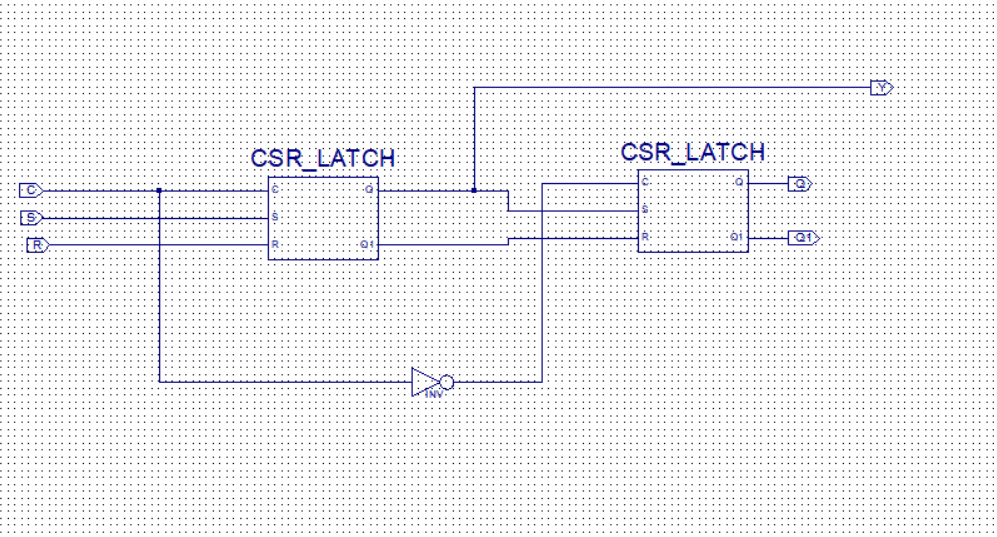
\includegraphics[width=0.9\textwidth]{lab9p/8.png}
    \caption{\label{Lab9}SR主从触发器}
    \end{figure}

\subsubsection*{SR主从触发器仿真代码initial块}
    \begin{figure}[H]
    \centering
    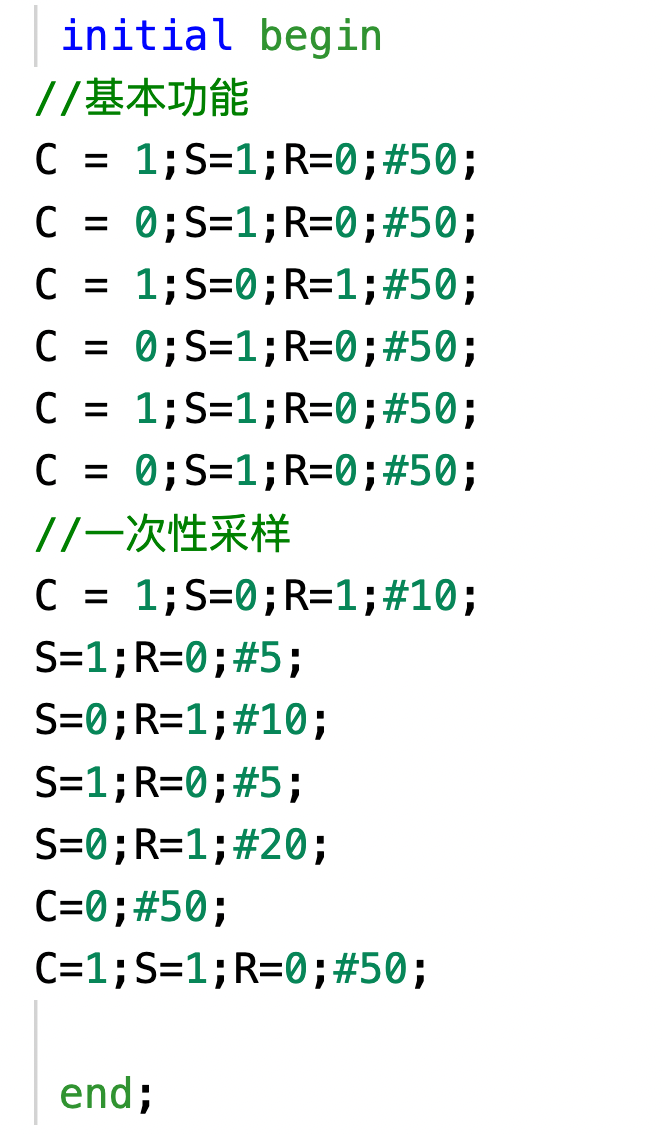
\includegraphics[width=0.3\textwidth]{lab9p/13.png}
    \caption{\label{Lab9}initial块}
    \end{figure}

\subsection*{5. D触发器}
    \begin{figure}[H]
    \centering
    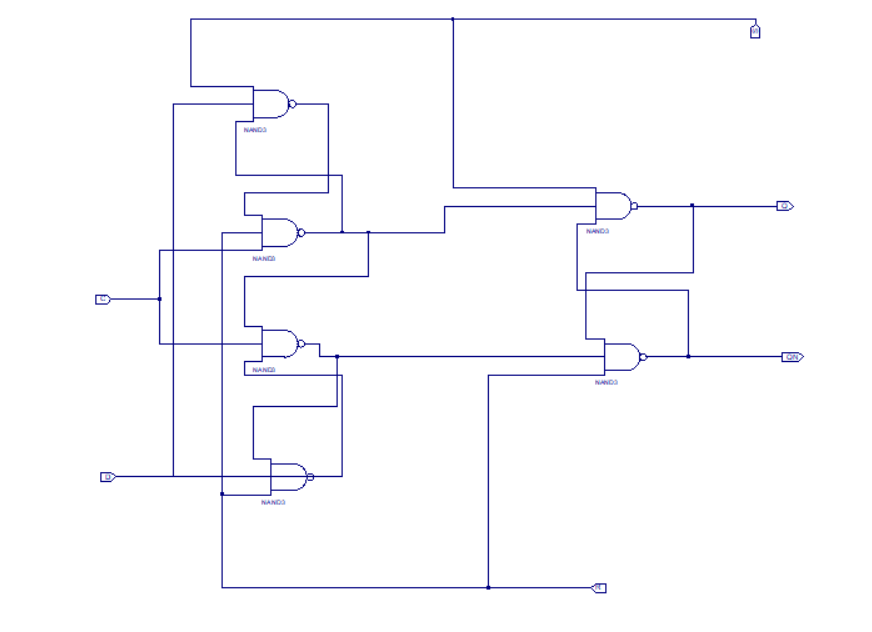
\includegraphics[width=0.9\textwidth]{lab9p/9.png}
    \caption{\label{Lab9}D触发器}
    \end{figure}

\subsubsection*{D触发器仿真代码initial块}
    \begin{figure}[H]
    \centering
    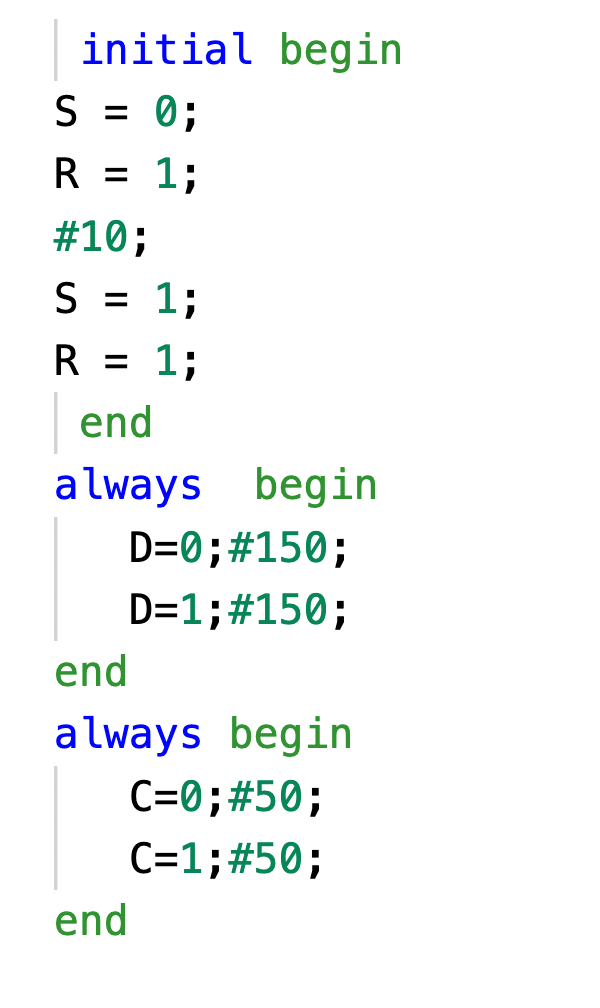
\includegraphics[width=0.3\textwidth]{lab9p/14.png}
    \caption{\label{Lab9}initial块}
    \end{figure}


\section*{二:实验结果与分析}

\subsection*{1. SR\_LATCH波形图与下板分析}
\subsubsection*{波形图:}    
    \begin{figure}[H]
    \centering
    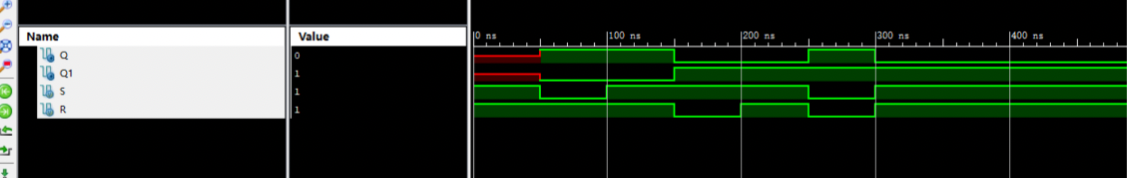
\includegraphics[width=1\textwidth]{lab9p/1.png}
    \caption{\label{Lab9}波形图}
    \end{figure}

\subsubsection*{波形图分析:}
S,R初始时都设置为1,为保持状态,但由于未设定初始值,因此显示为未定义态.

然后设置S=0,为置位(Set)状态,因此输出Q为1.接下来S=1,R=1,保持了这个状态.

设置R=0,为ReSet状态,输出Q为0.

当S=0,R=0时是一个未定义的状态,根据延时的长短会有一个状态显示出来,但实际上这种操作是不被允许的.



\subsection*{2. CSR\_LATCH波形图与下板分析}

\subsubsection*{波形图:}
    \begin{figure}[H]
    \centering
    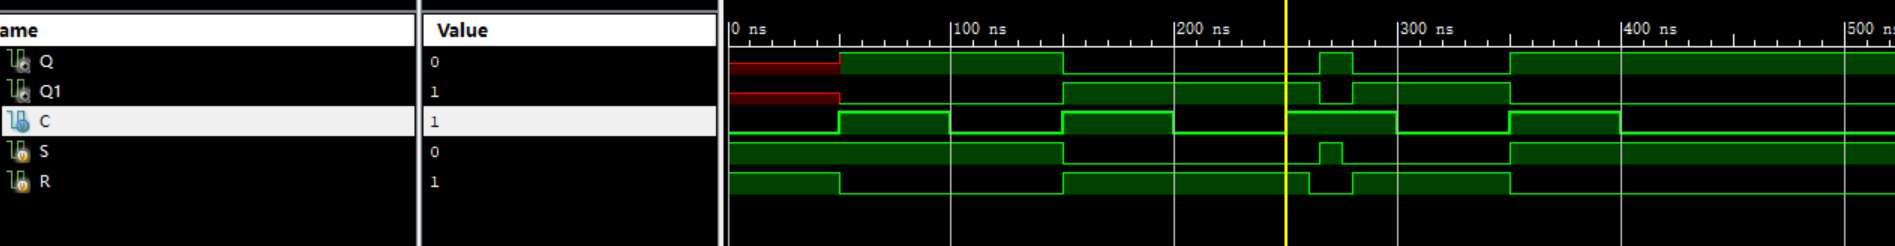
\includegraphics[width=1\textwidth]{lab9p/2.png}
    \caption{\label{Lab9}波形图}
    \end{figure}
\subsubsection*{波形图分析:}
在波形图中反应了CSR\_LATCH的空翻问题,信号C相当于时钟信号,当C=0时,会保持当前的状态不改变,
若C=1,则会根据S和R的输入进行结果的改变(S=1,置1 R=1,置0).

在波形图中可以看出"空翻"的问题:在C=1时如果S,R信号发生了多次的变化,那么对应的输出也会有多次的变化,在波形图中黄线以右
的一个脉冲可以看出这个问题.

\subsubsection*{下板图片:}
\subsubsection*{下板结果与分析:}
    \begin{figure}[H]
    \centering
    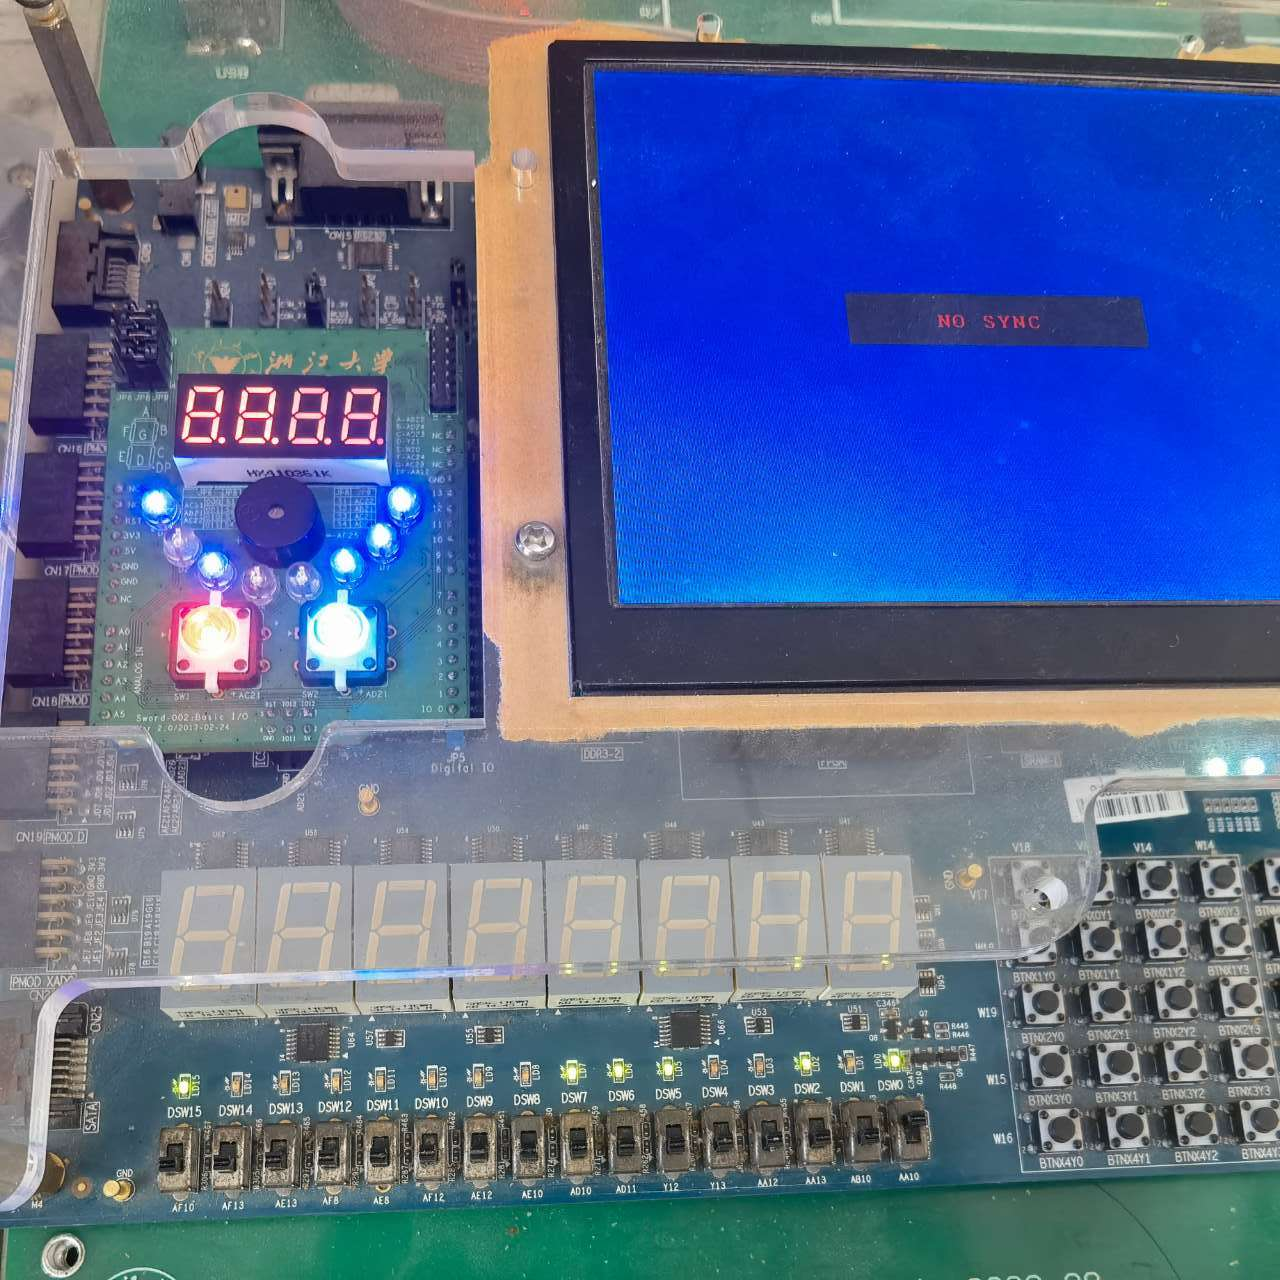
\includegraphics[width=0.5\textwidth]{lab9p/21.jpg}
    \caption{\label{Lab9}下板照片}
    \end{figure}

    \begin{figure}[H]
    \centering
    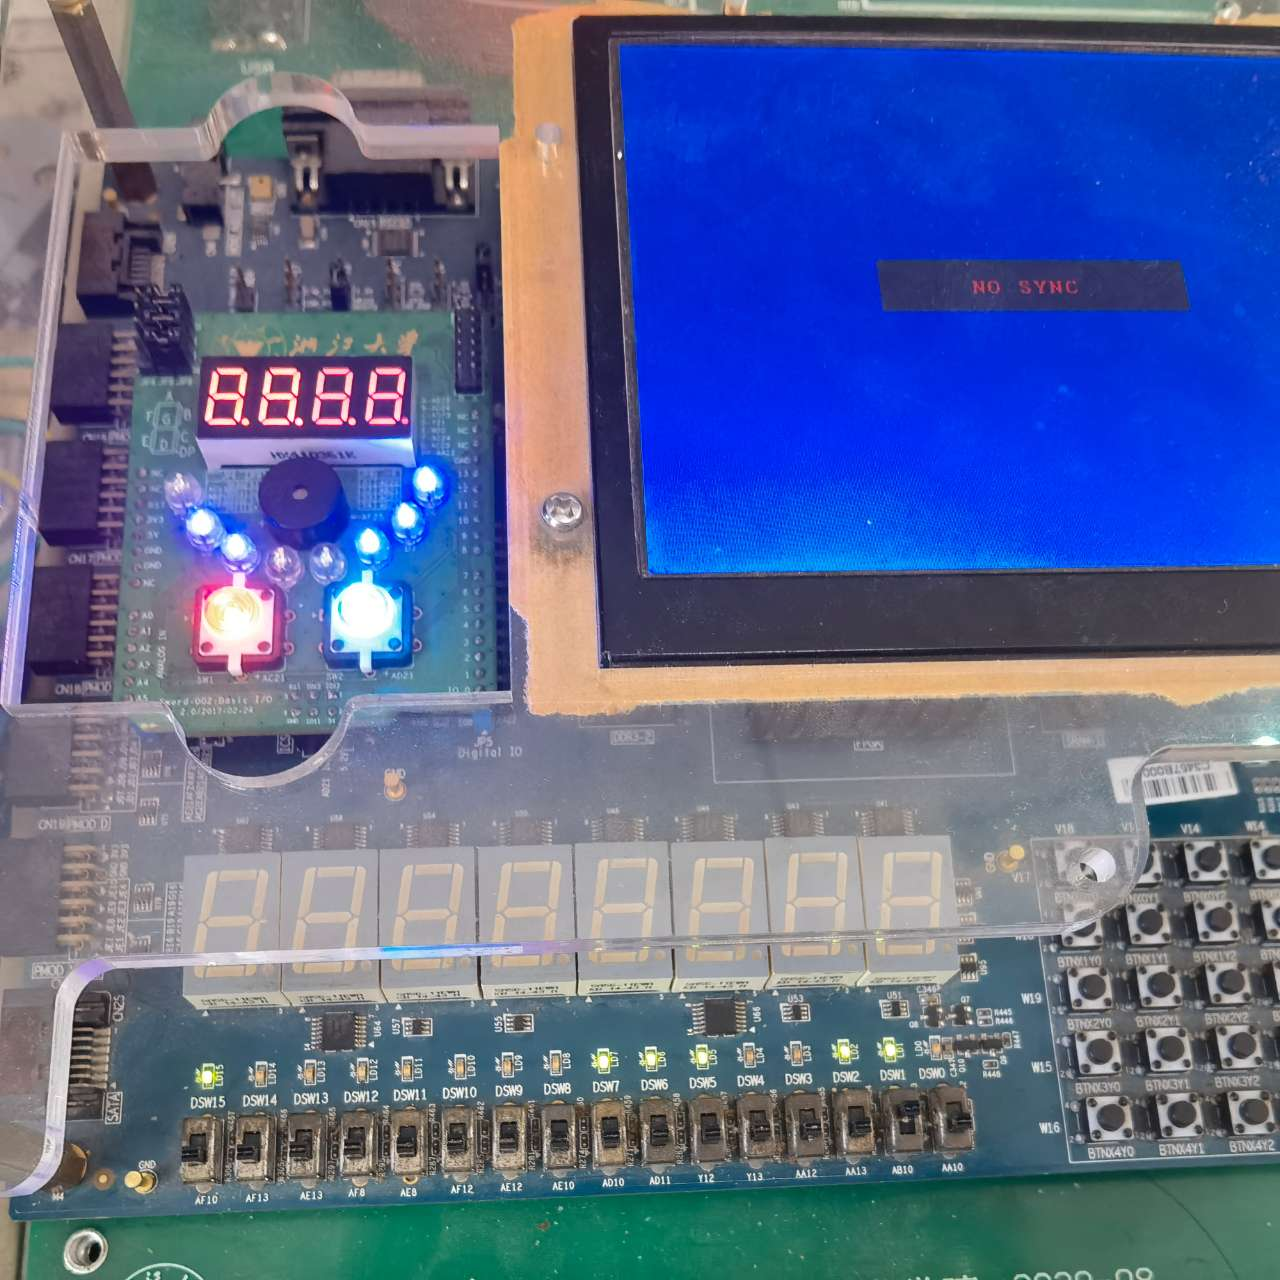
\includegraphics[width=0.5\textwidth]{lab9p/22.jpg}
    \caption{\label{Lab9}下板照片}
    \end{figure}

在自动时钟信号的情况下,当拨动S对应的开关时,对应Q的灯会闪亮,而Q\_bar熄灭.

拨动R对应的开关时,Q灯熄灭,Q\_bar闪亮.

调整为手动时钟信号时可以看出空翻的问题.

\subsection*{3. D\_LATCH 波形图与下板分析:}

\subsubsection*{波形图:}
    \subsubsection*{波形图:}
    \begin{figure}[H]
    \centering
    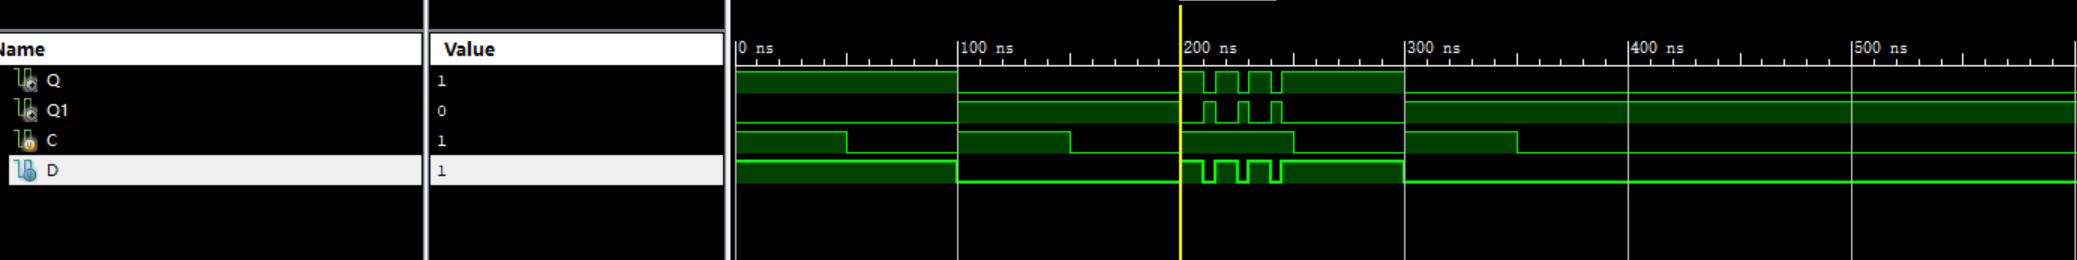
\includegraphics[width=1\textwidth]{lab9p/3.png}
    \caption{\label{Lab9}波形图}
    \end{figure}

\subsubsection*{波形图分析:}
信号C相当于时钟信号,当C=0时,会保持当前的状态不改变,
若C=1,则会根据D的输入进行结果的改变(D=1,置1 D=1,置0).

在波形图中可以看出D\_LATCH的空翻现象的问题,在黄线右侧的一个脉冲里,当C=1时,如果
D的信号有多次变化,那么对应的输出也会有多次的变化.


\subsubsection*{下板照片:}

    \begin{figure}[H]
    \centering
    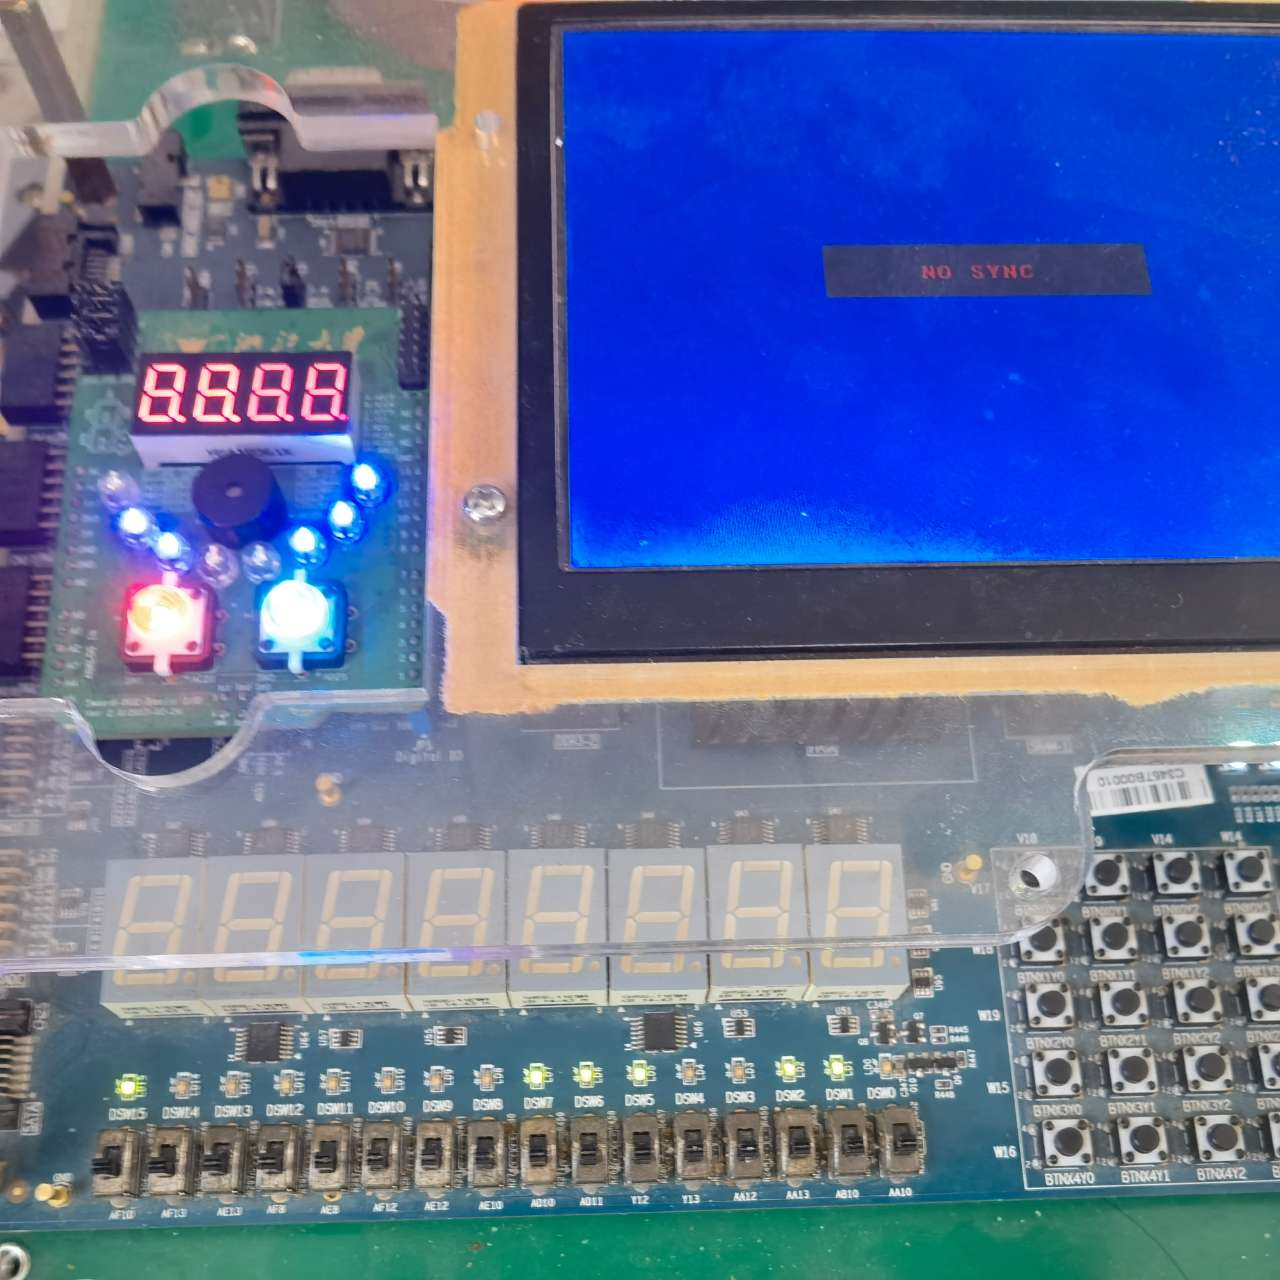
\includegraphics[width=0.5\textwidth]{lab9p/24.jpg}
    \caption{\label{Lab9}下板照片}
    \end{figure}

    \begin{figure}[H]
    \centering
    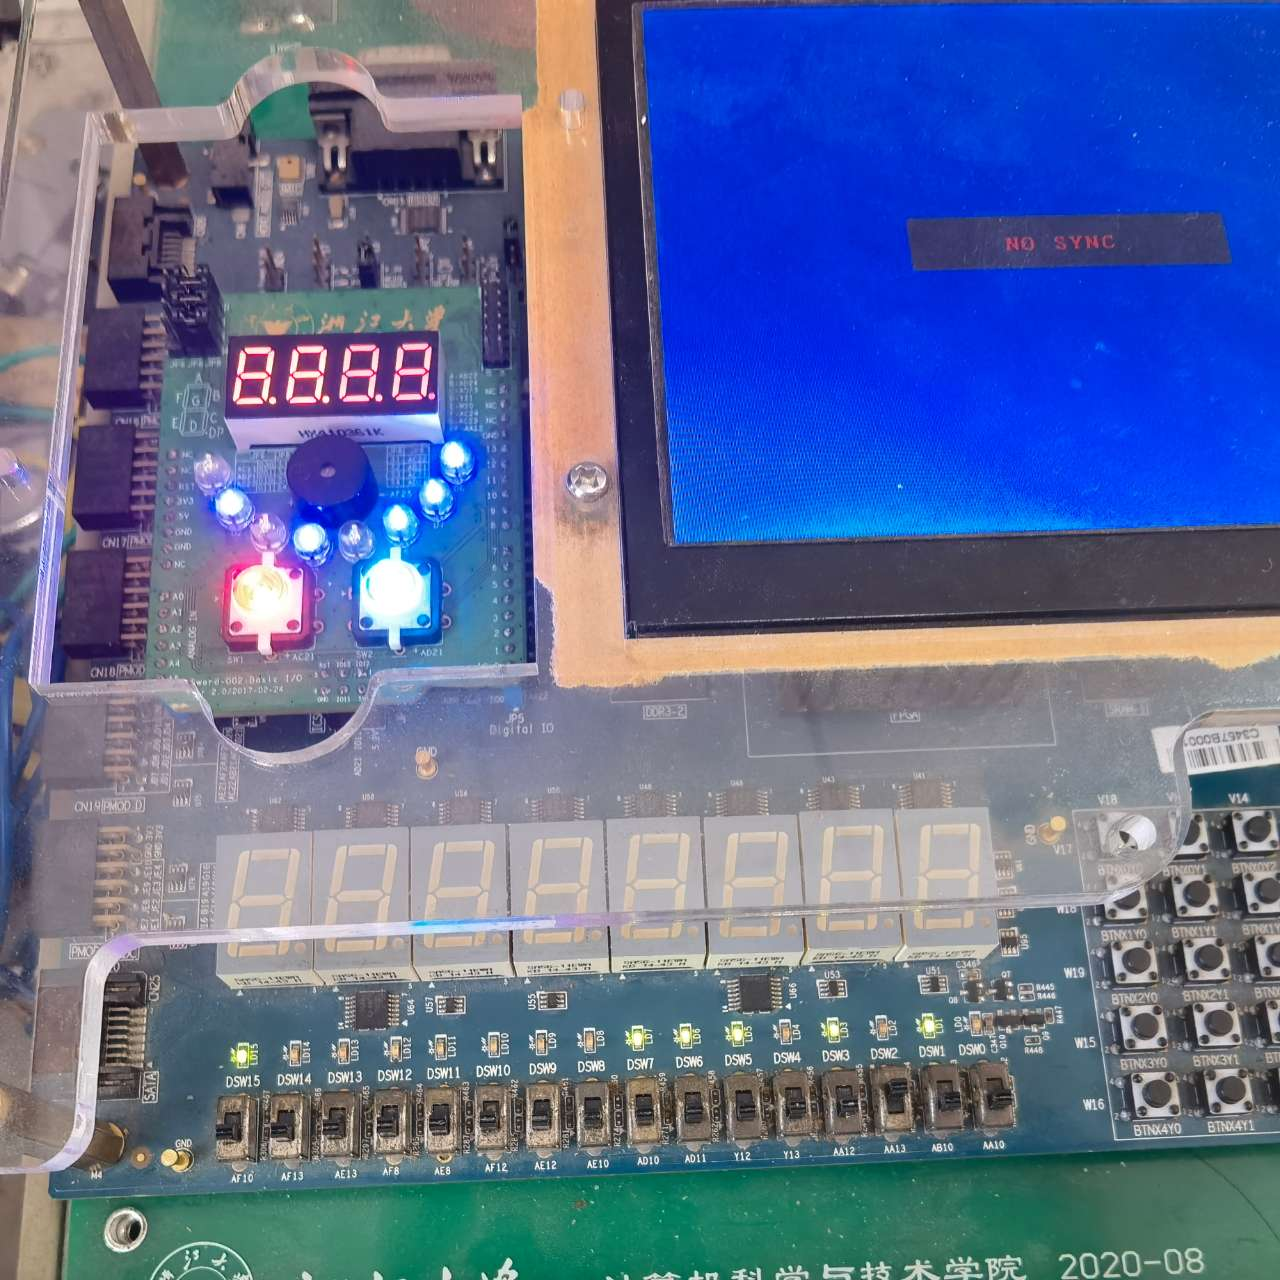
\includegraphics[width=0.5\textwidth]{lab9p/23.jpg}
    \caption{\label{Lab9}下板照片}
    \end{figure}

在自动时钟信号的条件下,如果开关D对应的开关被向上拨动时,对应的Q灯闪亮,Q\_bar熄灭.

关闭D对应的开关,Q灯熄灭,Q\_bar闪亮.

调整为手动时钟信号时可以看出空翻的问题.


\subsection*{4. SR主从触发器波形图与下板分析:}

\subsubsection*{波形图:}
    \begin{figure}[H]
    \centering
    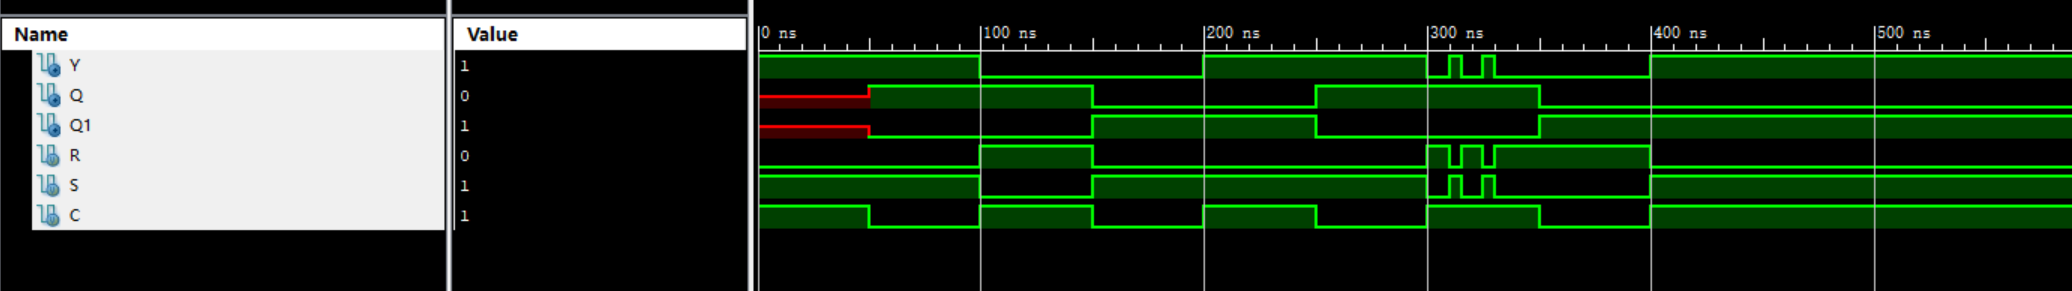
\includegraphics[width=1\textwidth]{lab9p/4.png}
    \caption{\label{Lab9}波形图}
    \end{figure}


\subsubsection*{波形图分析:}
这是一个负边沿SR主从触发器,当时钟信号为负时输出Q才会根据Y的输出而变化,而此时Y的信号不会发生改变.当时钟信号
为正时,会根据S和R的输入来改变对应Y的输出(若S=1,则Y=1. 若S=0,则Y=0).

在波形图中可以看出SR主从触发器的一次性采样的问题(300ns开始的一个脉冲),在时钟信号为正时,如果让S,R
输入的信号有多次的变化,那么对应的Y值会相应的有多次变化,但最终当时钟信号变为负时,输出Q只会显示最后
Y的结果,这会导致当有干扰信号发生时,会对干扰信号进行记录而产生错误.

\subsubsection*{下板照片:}
    \begin{figure}[H]
    \centering
    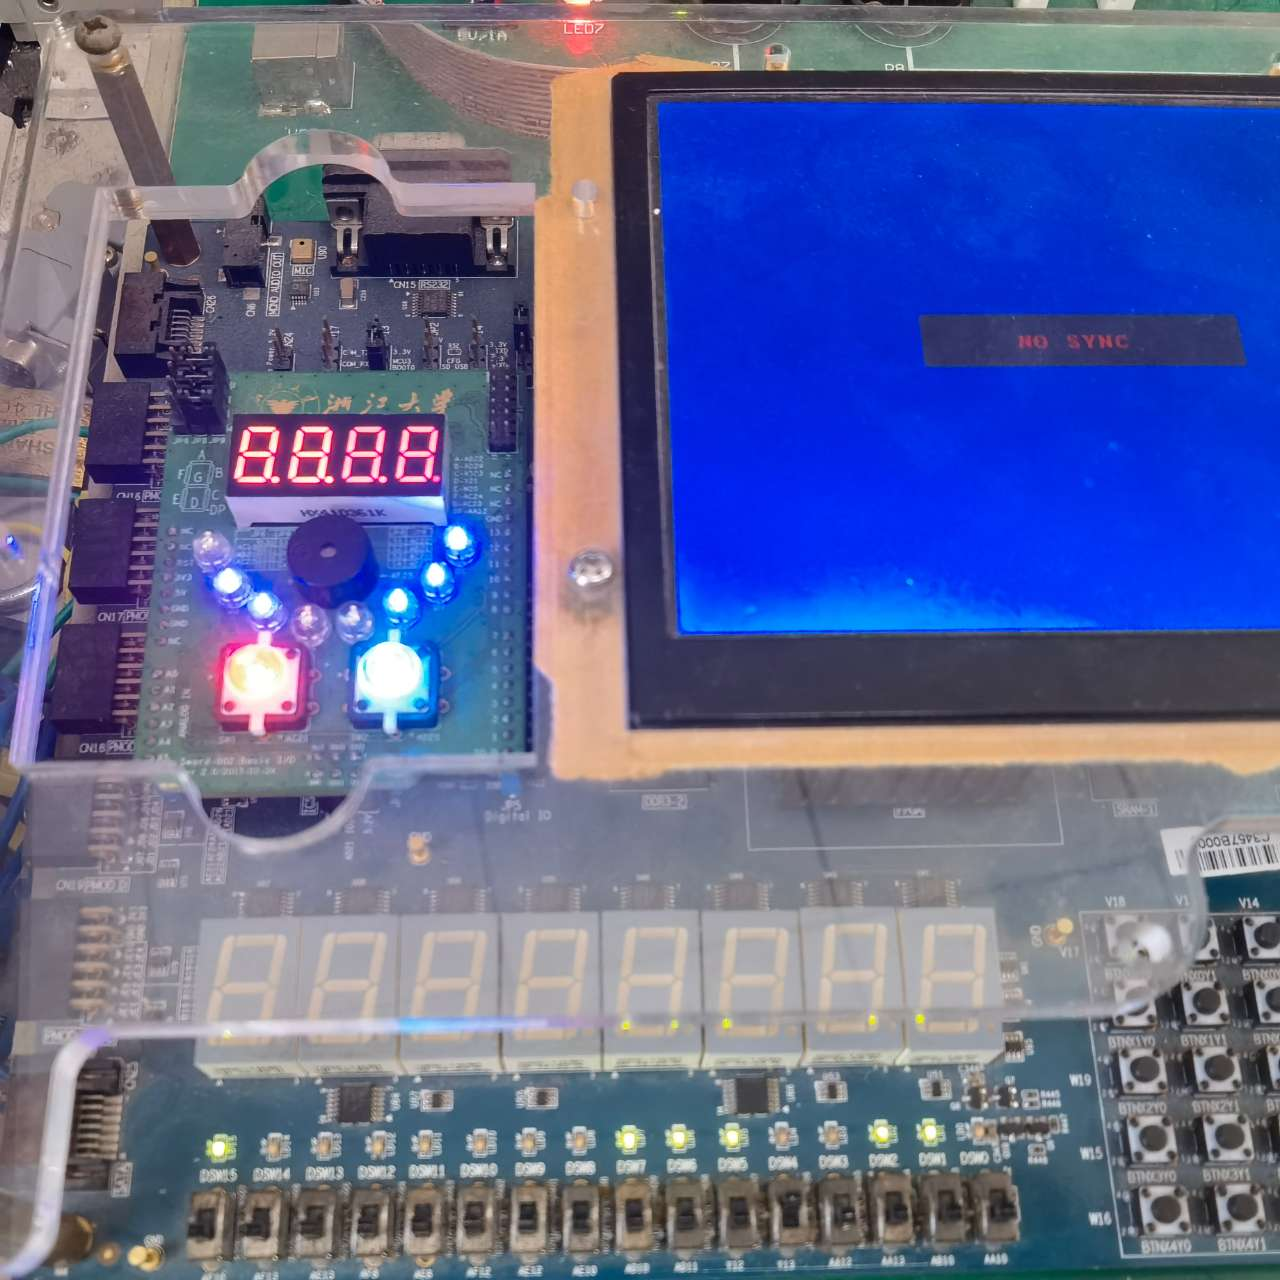
\includegraphics[width=0.5\textwidth]{lab9p/25.jpg}
    \caption{\label{Lab9}下板照片}
    \end{figure}

    \begin{figure}[H]
    \centering
    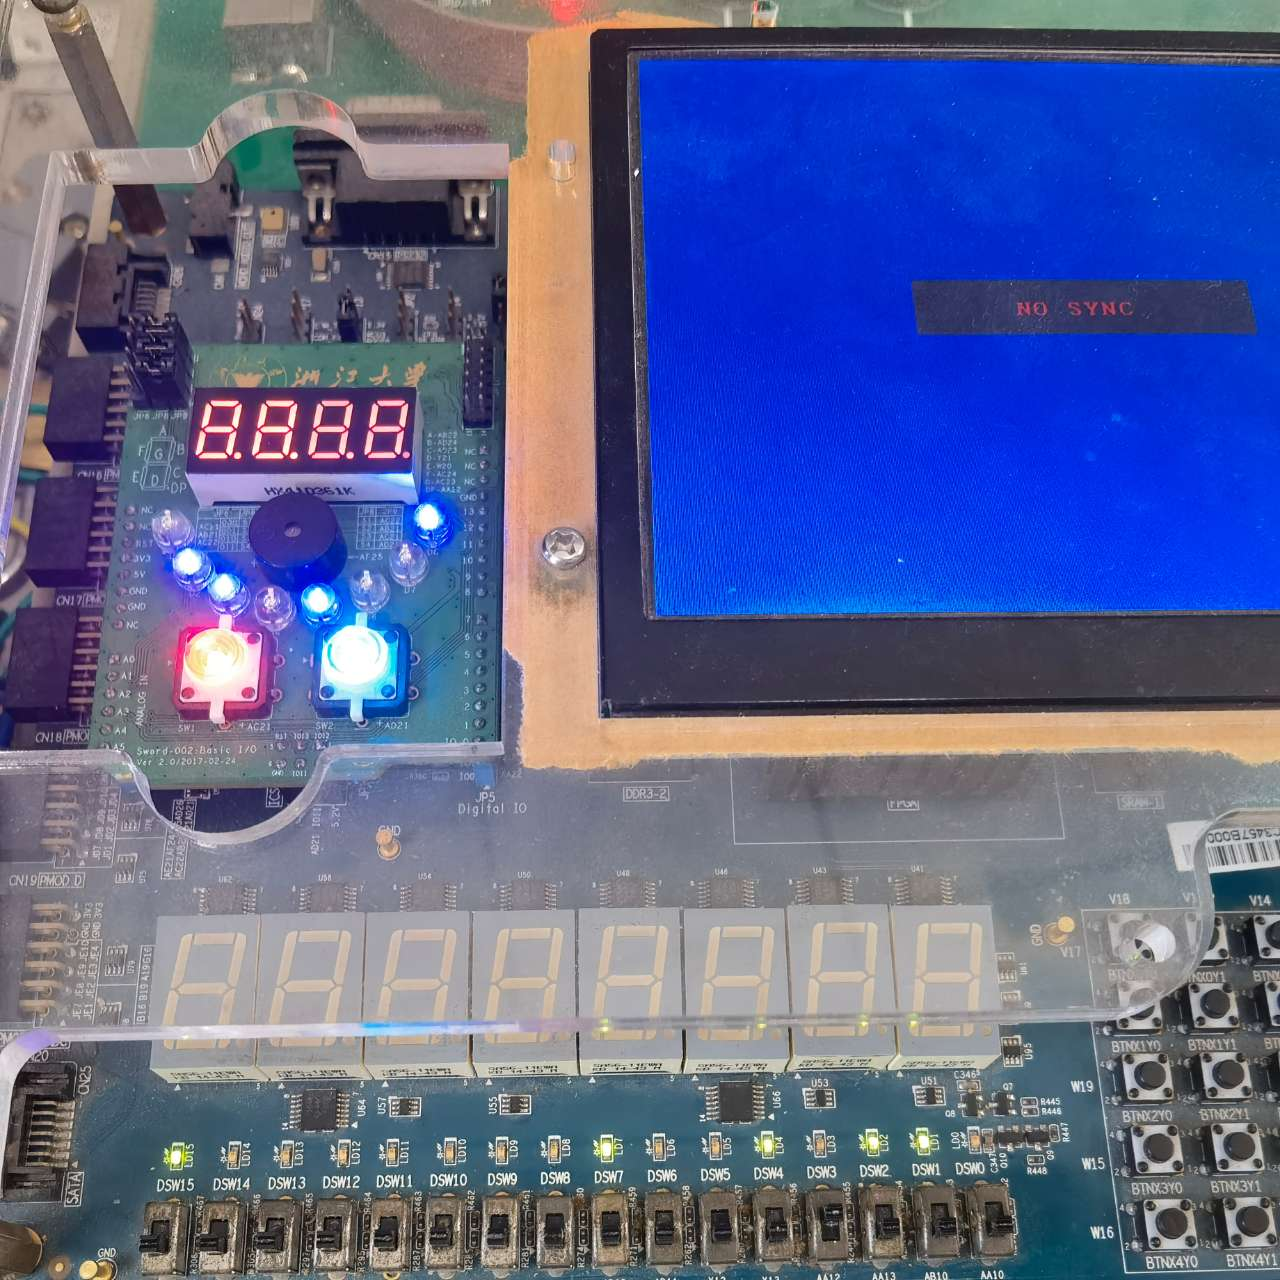
\includegraphics[width=0.5\textwidth]{lab9p/26.jpg}
    \caption{\label{Lab9}下板照片}
    \end{figure}

\subsection*{5. D触发器波形图与下版分析:}

在自动时钟信号时,拨动S对应的开关,当时钟信号为正时,Y对应的灯会先闪亮,然后时钟信号变为负时,
对应Q的灯会紧接着闪亮,因此可以看到在下板时两个灯是依次闪亮的并不是同时发生.

拨动R对应的开关,关闭S对应的开关,当时钟信号为正时,Y对应的灯会先熄灭,然后时钟信号变为负时,
Q对应的灯也熄灭,Q\_bar会闪亮.

调整为手动时钟信号时可以看出一次性采样的问题.

\subsubsection*{波形图:}
    \begin{figure}[H]
    \centering
    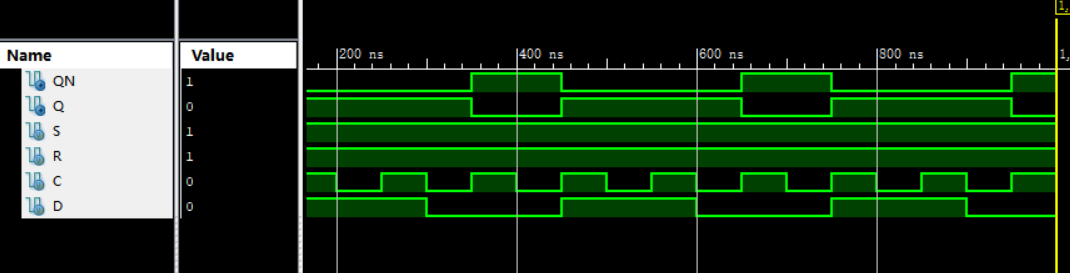
\includegraphics[width=1\textwidth]{lab9p/10.png}
    \caption{\label{Lab9}波形图}
    \end{figure}


\subsubsection*{波形图分析:}



S,R的信号起到的是初始化置位的作用,D触发器当时钟信号为正时输出信号会根据D的信号发生相应的改变,
若D=1,则输出Q=1 . 若D=0,则输出Q=0. 若时钟信号为负,那么输出信号将不会发生改变.

\subsubsection*{下板照片:}

\begin{figure}[H]
    \centering
    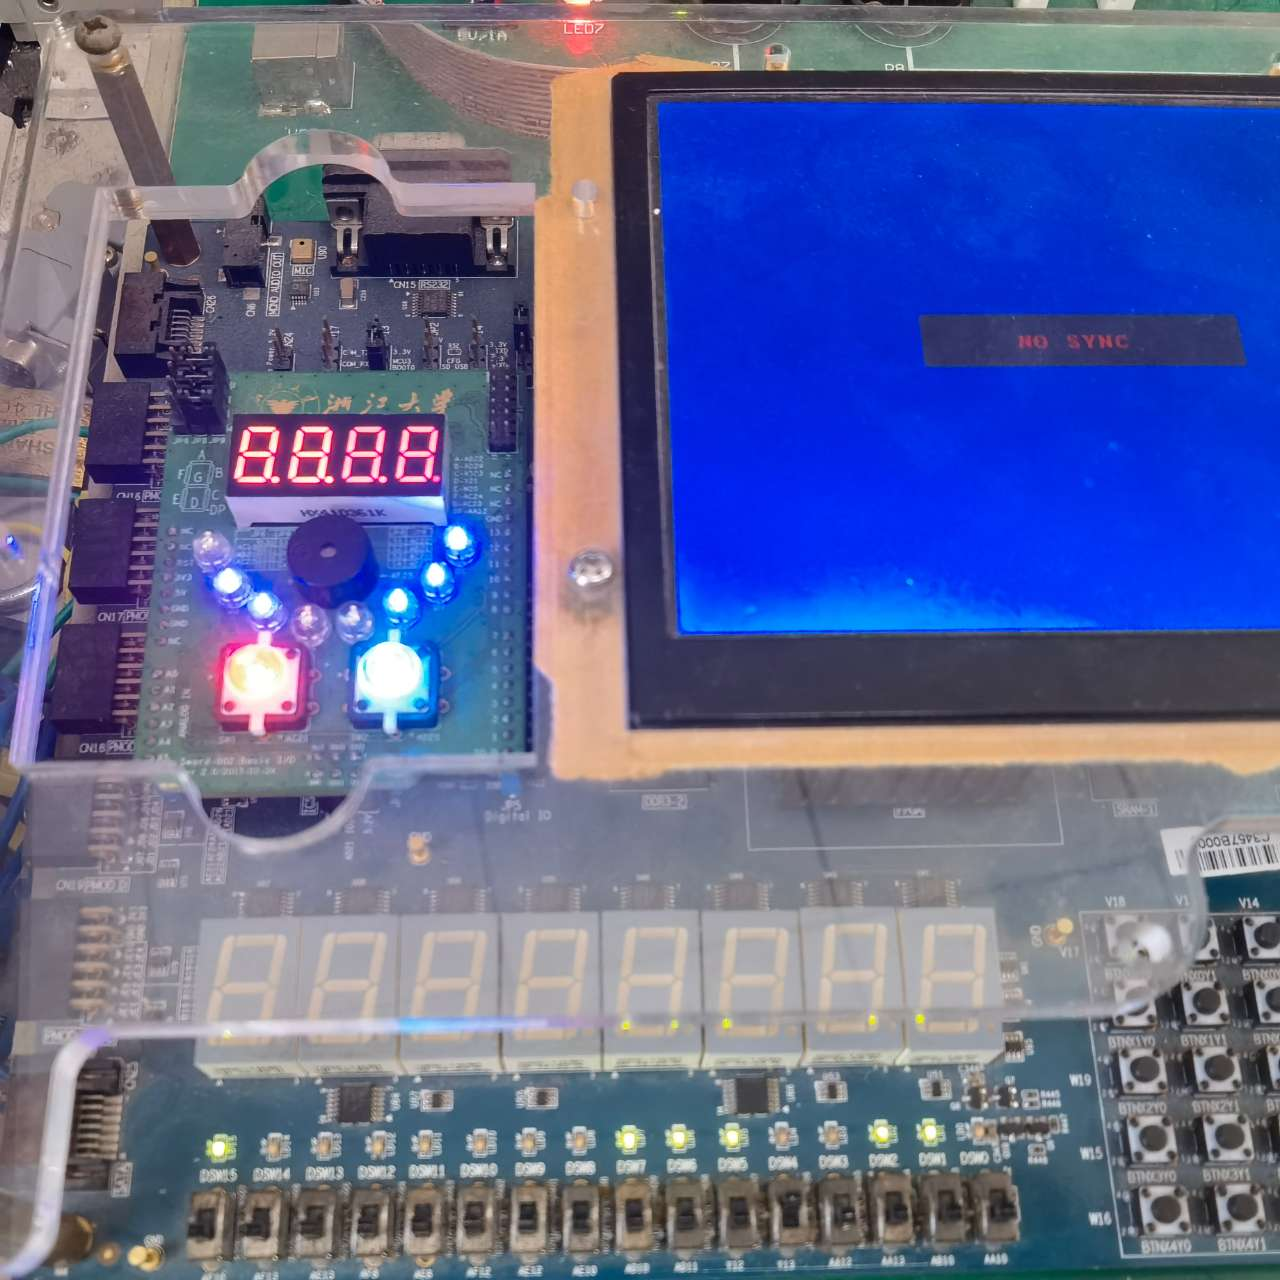
\includegraphics[width=0.5\textwidth]{lab9p/25.jpg}
    \caption{\label{Lab9}下板照片}
    \end{figure}

    \begin{figure}[H]
    \centering
    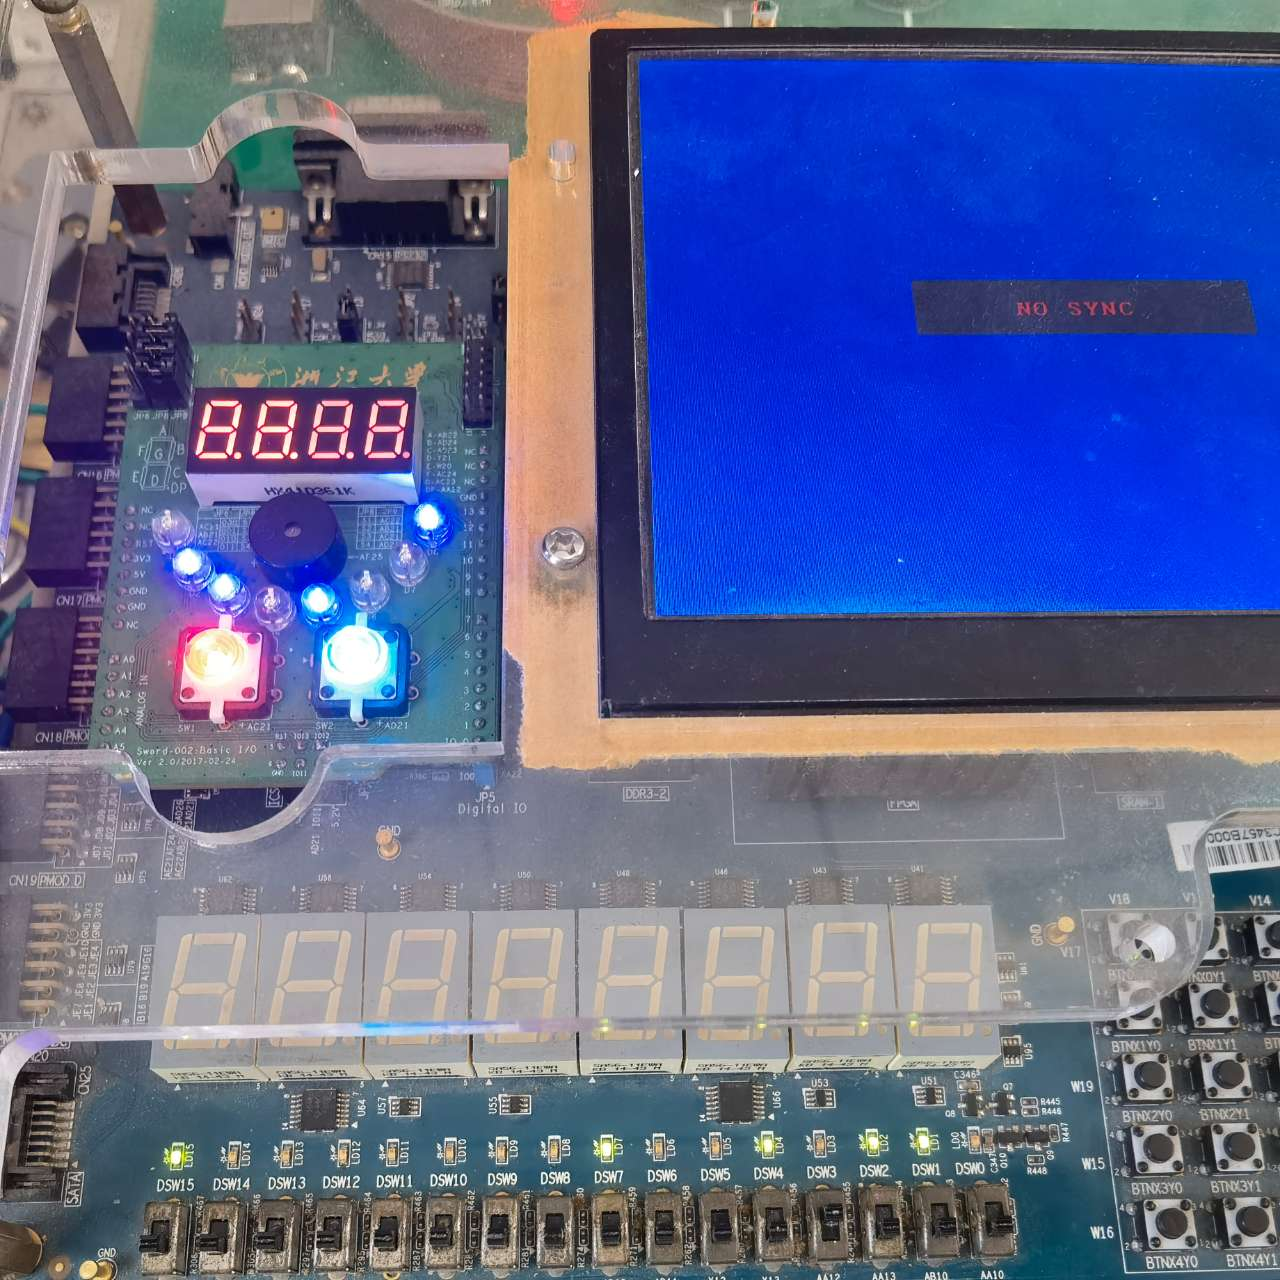
\includegraphics[width=0.5\textwidth]{lab9p/26.jpg}
    \caption{\label{Lab9}下板照片}
    \end{figure}

在自动时钟信号的情况下,当拨动D对应的开关时,Q对应的灯闪亮.

关闭D对应的开关,Q对应的灯熄灭.


\section*{三:讨论与心得}

本次实验遇到的主要问题是,一开始没有找到手动时钟信号对应的按钮,因此在用过下板
验证空翻问题和一次性采样时没有找到合适的方法,理解了手动时钟信号的控制原理之后
才得以验证.

\end{document}